The results vary somewhat widely with the bug analyzed and the automated diversity implementation used.

Applying implementation 1 (interposition of all external library function calls) to Libsafe resulted in a dramatic decrease in exploit success rate with increasing microbenchmark overhead (Figures \ref{fig_libsafe-all} and \ref{fig_libsafe-all-zoom}).
Between 1x overhead and 12x overhead, no randomizations resulted in less than a 5\% success rate.
Between 20x and 25x overhead, 27.5\% of randomizations resulted in less than a 5\% exploit success rate.
Between 40x and 45x overhead, 61.5\% of randomizations resulted in less than a 5\% exploit success rate.
Beyond 1,040x overhead, 100\% of randomizations resulted in less than a 5\% exploit success rate.
\begin{figure}
	\centering
	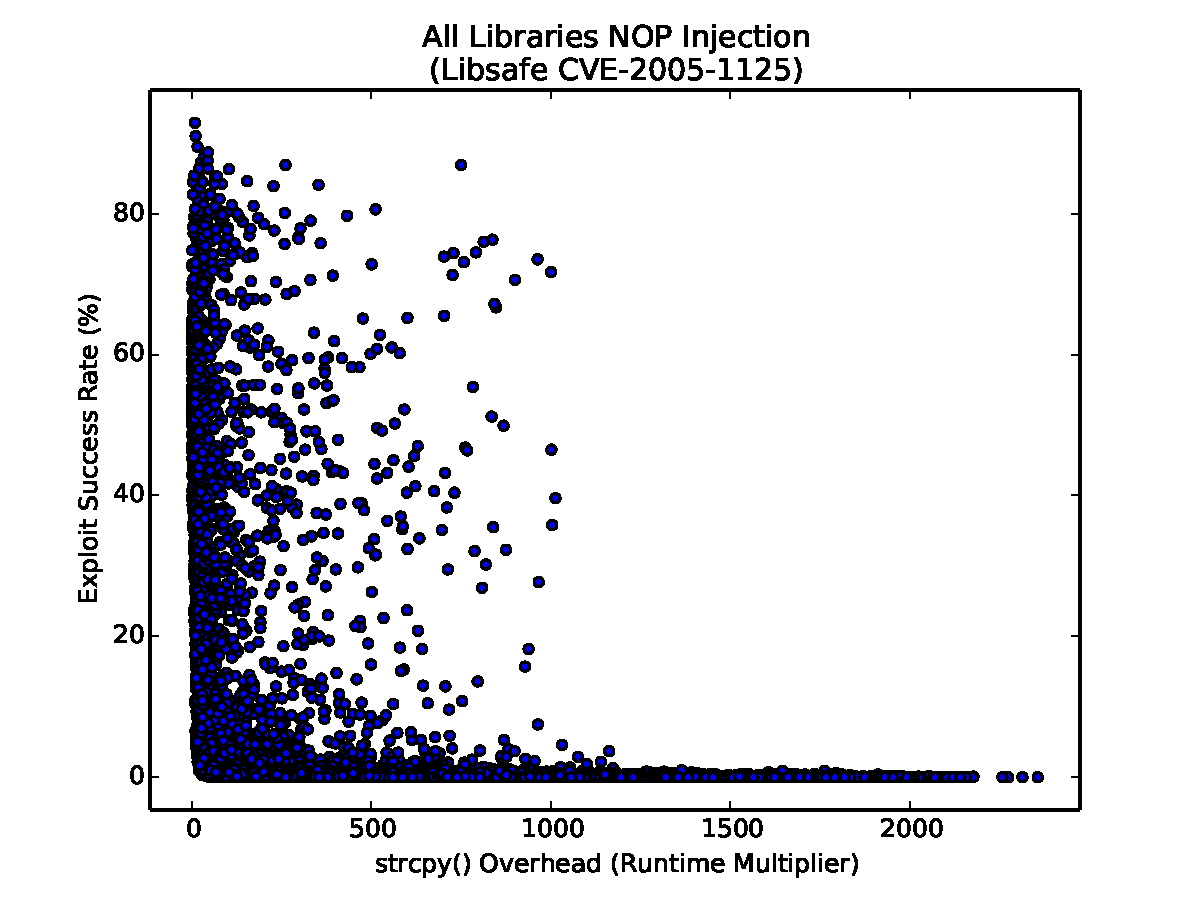
\includegraphics[width=\columnwidth]{figures/libsafe-all}
	\caption{Exploit success rate as a function of the microbenchmark after applying diversity implementation 1 to Libsafe with concurrency bug CVE-2005-1125.}
	\label{fig_libsafe-all}
\end{figure}
\begin{figure}
	\centering
	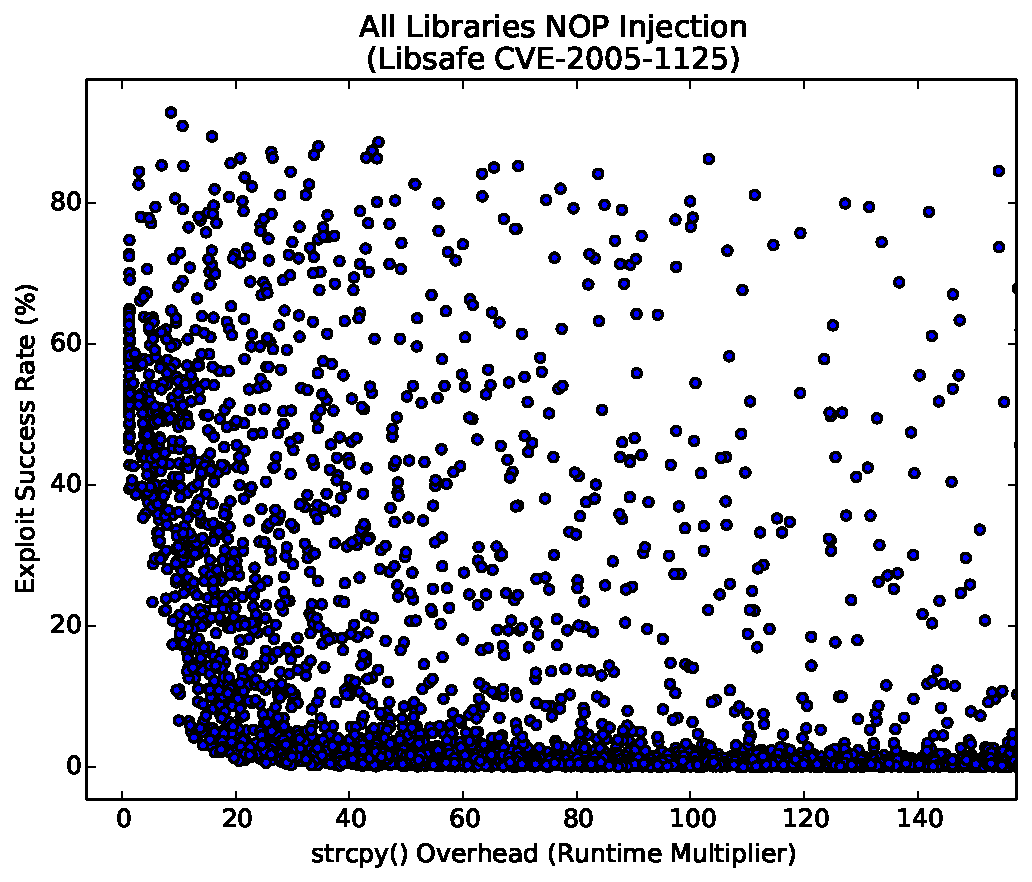
\includegraphics[width=\columnwidth]{figures/libsafe-all-zoom}
	\caption{Exploit success rate as a function of the microbenchmark after applying diversity implementation 1 to Libsafe with concurrency bug CVE-2005-1125 (a zoom-in of Figure \ref{fig_libsafe-all}).}
	\label{fig_libsafe-all-zoom}
\end{figure}

Applying implementation 2 to Libsafe had no noticeable effect on exploit success rate (Figure \ref{fig_libsafe-pre}) or microbenchmark overhead.
\begin{figure}
	\centering
	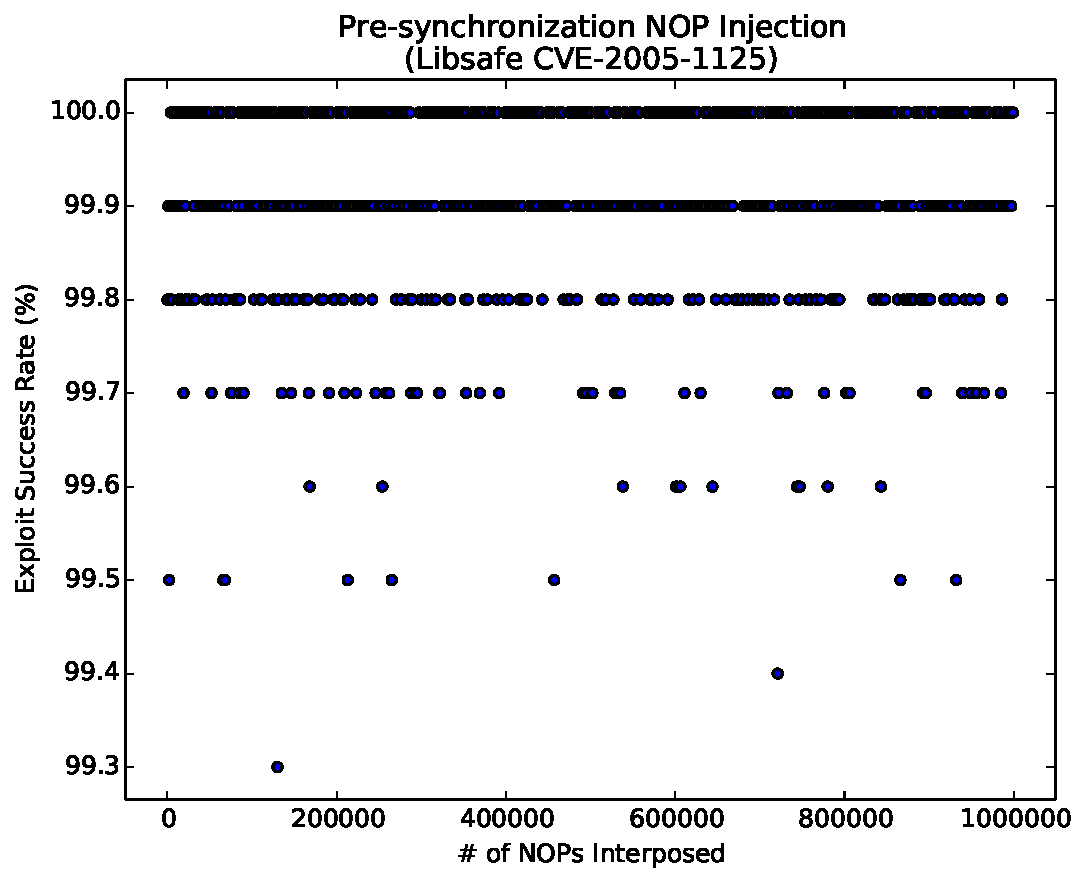
\includegraphics[width=\columnwidth]{figures/libsafe-pre}
	\caption{Exploit success rate as a function of the microbenchmark after applying diversity implementation 2 to Libsafe with concurrency bug CVE-2005-1125.}
	\label{fig_libsafe-pre}
\end{figure}

Applying implementation 3 to Libsafe had a very marked effect on exploit success rate (Figure \ref{fig_libsafe-post}).
In particular, exploit success rate remains high for low numbers of NOPs.
Then, for inserted NOP loops of lengths greater than 200,000, exploit success rate begins to drop.
For inserted NOP loops of lengths between 250,000 and 350,000, exploit success rate fluctuates between 35\% and 65\%.
Finally, for inserted NOP loops of lengths greater than 350,000, exploit rates drop even further, and beyond loop-lengths of 390,000 NOPs, all interpositions resulted in exploit rates less than 0.5\%.
\begin{figure}
	\centering
	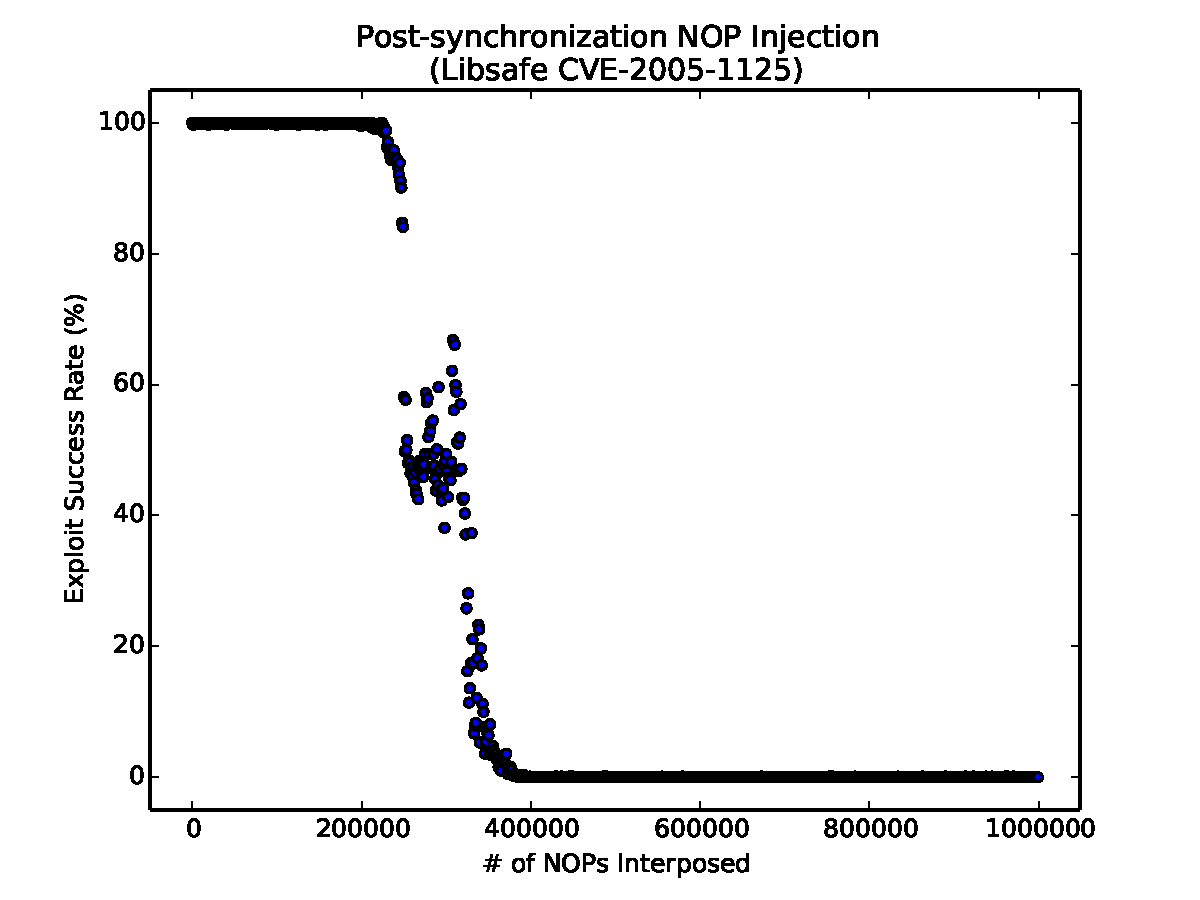
\includegraphics[width=\columnwidth]{figures/libsafe-post}
	\caption{Exploit success rate as a function of the number of NOPs injected after applying diversity implementation 3 to Libsafe with concurrency bug CVE-2005-1125.}
	\label{fig_libsafe-post}
\end{figure}


\begin{figure}
	\centering
	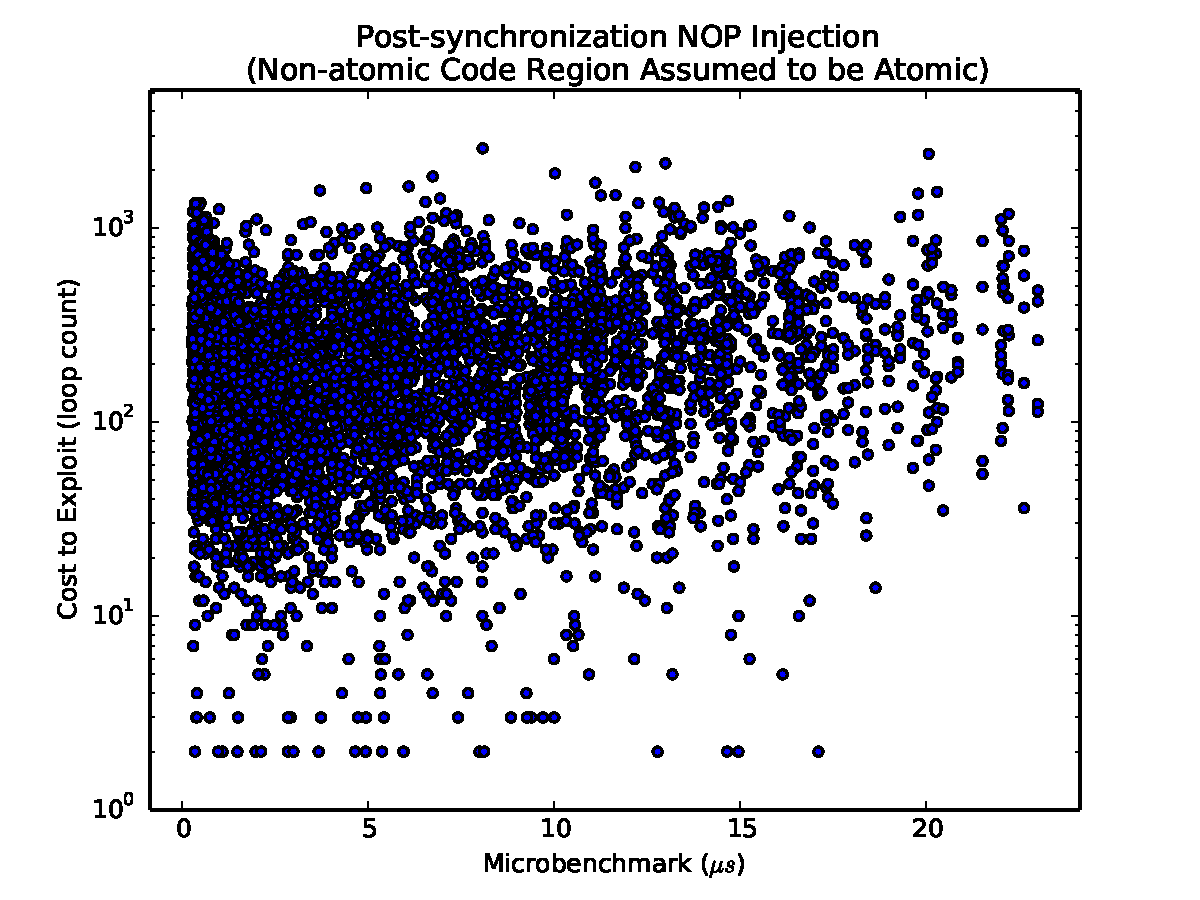
\includegraphics[width=\columnwidth]{figures/nonatomic-post}
	\caption{Exploit cost (in number of exploit attempts) as a function of the microbenchmark after applying diversity implementation 3 to a canonical "nonatomic-region-assumed-to-be-atomic" concurrency bug.}
	\label{fig_nonatomic-post}
\end{figure}







\begin{figure}
	\centering
	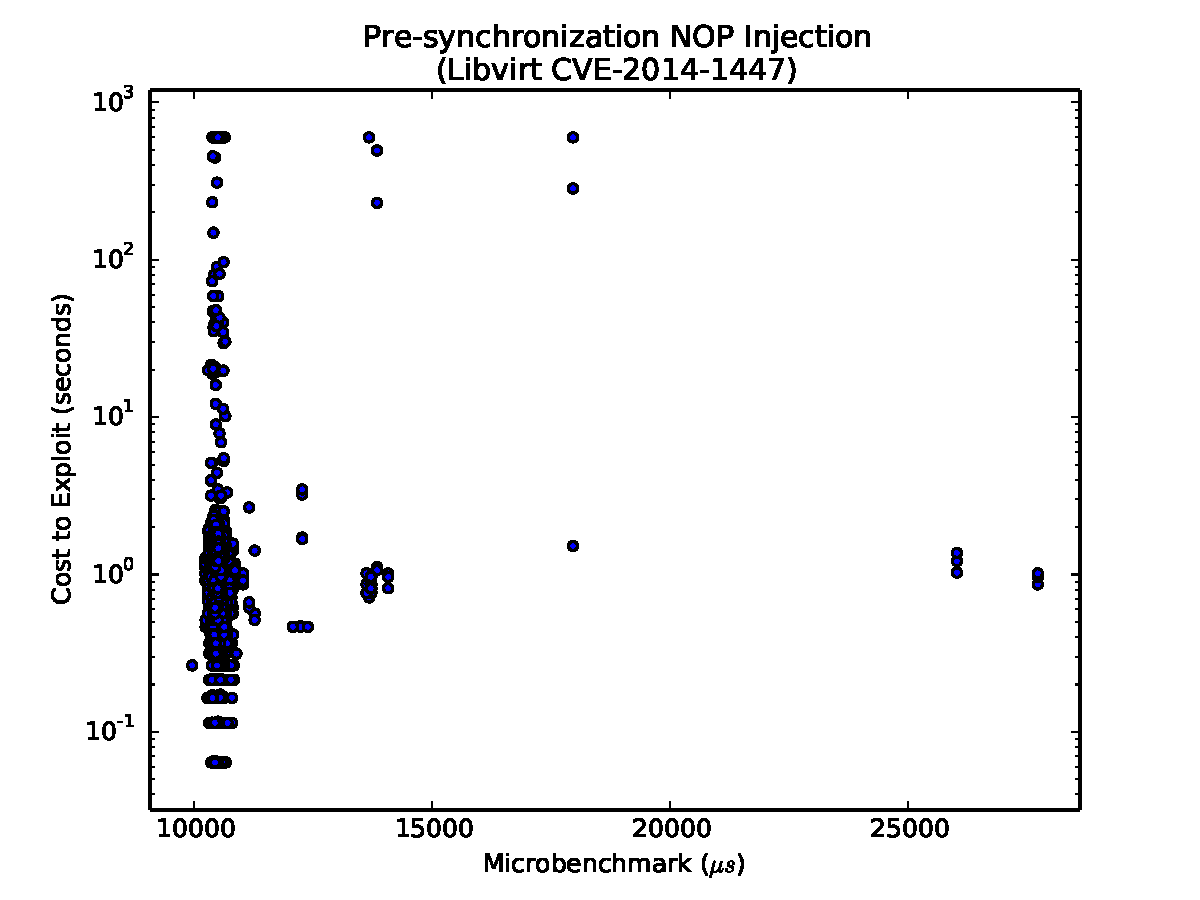
\includegraphics[width=\columnwidth]{figures/libvirt-pre}
\caption{Exploit cost (in time) as a function of the microbenchmark after applying diversity implementation 2 to Libvirt with concurrency bug CVE-2014-1447.}
	\label{fig_libvirt-pre}
\end{figure}

\begin{figure}
	\centering
	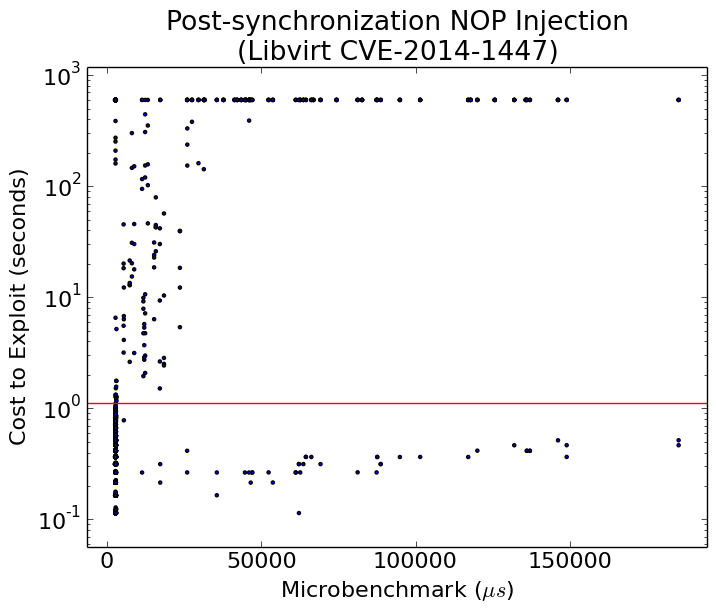
\includegraphics[width=\columnwidth]{figures/libvirt-post}
\caption{Exploit cost (in time) as a function of the microbenchmark after applying diversity implementation 3 to Libvirt with concurrency bug CVE-2014-1447.}
	\label{fig_libvirt-post}
\end{figure}